\documentclass[aspectratio=169,10pt]{beamer}
\usetheme{moloch}
\molochset{progressbar=frametitle, titleformat=regular}
\setbeamertemplate{page number in head/foot}[totalframenumber]
\molochset{block=fill}
\usepackage{standalone}
\usepackage[T1]{fontenc}
\usepackage[utf8]{inputenc}
\usepackage{lmodern}
\usepackage{amsmath,amssymb}
\usepackage{booktabs,tabularx,array}
\usepackage{graphicx}
\usepackage{xcolor}
\usepackage{ragged2e}
\usepackage{tikz}
\usepackage{fontawesome5}
\usepackage{fancyqr}

\pdfstringdefDisableCommands{%
  \def\translate#1{#1}%
}

\usetikzlibrary{positioning,arrows.meta,fit,backgrounds,calc}

\graphicspath{{assets/}}
\setlength{\tabcolsep}{5pt}
\renewcommand{\arraystretch}{1.12}

\title{Storytelling as Inverse Inverse Planning}
\subtitle{Chandra, Li, Tenenbaum \& Ragan-Kelley (2023) --- with Borges, \emph{The Garden of Forking Paths}}
\author{Aldo Costa}
\institute{Master-Seminar: Theory of Mind}
\date{21.01.27}

% --------------------------------------------------
% Semantic colours
% --------------------------------------------------
\definecolor{robotBlue}{HTML}{4C78A8}
\definecolor{cheeseGold}{HTML}{C9A100}
\definecolor{goalPink}{HTML}{D6409F}
\definecolor{goalGreen}{HTML}{3E9B4F}
\definecolor{beliefPurple}{HTML}{8E5BA8}
\definecolor{tellerOrange}{HTML}{E07B2E}
\definecolor{borgesRed}{HTML}{B5443A}
\definecolor{softGray}{HTML}{F2F3F3}

\newcommand{\robot}[1]{\textcolor{robotBlue}{#1}}
\newcommand{\cheese}[1]{\textcolor{cheeseGold!85!black}{#1}}
\newcommand{\pink}[1]{\textcolor{goalPink}{#1}}
\newcommand{\green}[1]{\textcolor{goalGreen}{#1}}
\newcommand{\belief}[1]{\textcolor{beliefPurple}{#1}}
\newcommand{\teller}[1]{\textcolor{tellerOrange}{#1}}
\newcommand{\borges}[1]{\textcolor{borgesRed}{#1}}
\newcommand{\Prob}{\mathrm{P}}

\newcommand{\figsource}[1]{\par\vspace{0.2em}{\centering\tiny\color{gray}#1\par}}
\newcommand{\tightitem}{\itemsep0.3em}
\newcommand{\slideendspace}{\vspace{0.3em}}

% Placeholder-safe figure include.
% Put cropped paper figures as PDFs in assets/.
\newcommand{\paperfig}[2][0.52]{%
\IfFileExists{assets/#2.pdf}{%
  \includegraphics[width=\linewidth,height=#1\textheight,keepaspectratio]{#2.pdf}%
}{%
  \begin{center}
  \fbox{%
    \begin{minipage}[c][#1\textheight][c]{0.92\linewidth}
    \centering
    \small Figure placeholder:\\[0.4em]
    \texttt{\detokenize{assets/#2.pdf}}
    \end{minipage}
  }
  \end{center}
}%
}

\begin{document}

\begin{frame}[plain]
\titlepage

\begin{tikzpicture}[remember picture,overlay]
\node[
  anchor=south east,
  xshift=-0.85cm,
  yshift=0.65cm
] at (current page.south east) {
  \begin{minipage}{2.4cm}
  \centering
  \fancyqr[
    size=2.4cm,
    color=black,
    level=H,
    tight
  ]{https://github.com/Eyecatch3r/storytelling-inverse-inverse-planning-seminar}\\[-0.05em]
  {\scriptsize Scan for notes and slides}
  \end{minipage}
};
\end{tikzpicture}

\end{frame}

% ==================================================
\section{Motivation}
% ==================================================

\begin{frame}{Two triangles and a circle}
\begin{columns}[T,onlytextwidth]

\begin{column}{0.48\textwidth}
\begin{block}{\faFilm\ Heider \& Simmel (1944)}
A 90-second animation of simple shapes moving on a plane.
\begin{itemize}\tightitem
  \item viewers see \alert{agents with goals}
  \item they judge characters as bully, victim, hero
  \item no faces, no words --- only motion
\end{itemize}
\end{block}
\end{column}

\begin{column}{0.48\textwidth}
\begin{block}{\faRobot\ Can a computer do this?}
First try: simulate rational agents with a planner.
\begin{itemize}\tightitem
  \item the agents reach their goals
  \item but the animation is \alert{flat}
  \item no suspense, no surprise, no irony
\end{itemize}
\end{block}
\end{column}

\end{columns}

\slideendspace
\begin{alertblock}{\faLightbulb\ Question of the paper}
What does a storyteller do that a rational agent does not?
\end{alertblock}
\end{frame}

\begin{frame}{Acting \emph{in} vs.\ acting \emph{out} a situation}
\begin{columns}[T,onlytextwidth]

\begin{column}{0.48\textwidth}
\begin{block}{\faWalking\ Acting \emph{in} a situation}
\centering
\textbf{Optimize the character's reward}
\end{block}
\begin{itemize}\tightitem
  \item agent wants to reach a goal
  \item best action = shortest path to the goal
\end{itemize}
\end{column}

\begin{column}{0.48\textwidth}
\begin{block}{\faTheaterMasks\ Acting \emph{out} a situation}
\centering
\textbf{Optimize the audience's belief}
\end{block}
\begin{itemize}\tightitem
  \item storyteller wants the audience to \emph{infer} a goal
  \item best action can be \alert{sub-optimal} in the world
\end{itemize}
\end{column}

\end{columns}

\slideendspace
\begin{alertblock}{\faBook\ Stories as ``probability design'' (Kukkonen, 2014)}
A story is a sequence of observations that moves the reader's beliefs over time.
\alert{Good stories design the journey of those beliefs.}
\end{alertblock}
\end{frame}

% ==================================================
\section{Background}
% ==================================================

\begin{frame}{Planning, inverse planning, inverse inverse planning}
\centering
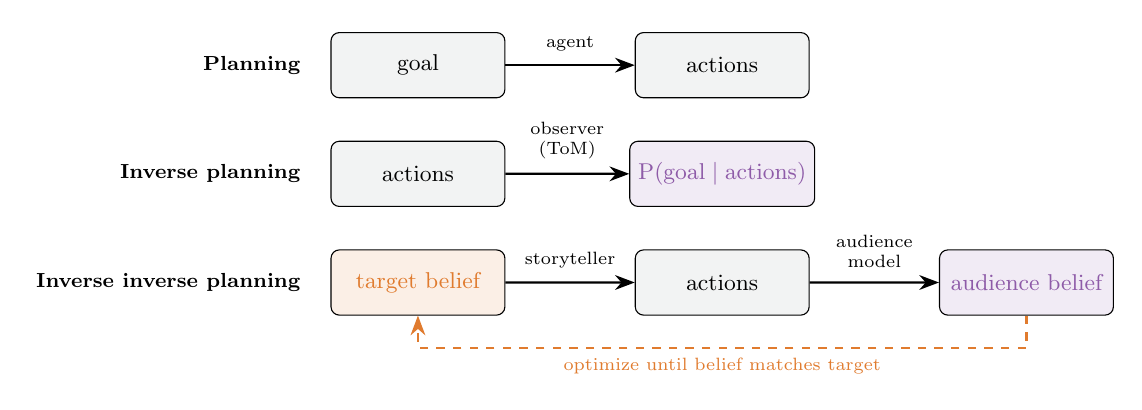
\begin{tikzpicture}[
  font=\small,
  box/.style={draw, rounded corners=3pt, minimum width=2.4cm, minimum height=0.9cm, align=center, fill=softGray},
  arr/.style={-{Stealth[length=2.5mm]}, thick},
  arrlab/.style={above=2pt, font=\scriptsize, align=center},
  scale=0.92, transform shape,
  lab/.style={font=\footnotesize\bfseries, anchor=east}
]
  % planning
  \node[lab] at (-0.2,0) {Planning};
  \node[box] (g1) at (1.3,0) {goal};
  \node[box] (a1) at (5.5,0) {actions};
  \draw[arr] (g1) -- node[arrlab]{agent} (a1);

  % inverse planning
  \node[lab] at (-0.2,-1.5) {Inverse planning};
  \node[box] (a2) at (1.3,-1.5) {actions};
  \node[box, fill=beliefPurple!12] (b2) at (5.5,-1.5) {\belief{$\Prob(\text{goal}\mid\text{actions})$}};
  \draw[arr] (a2) -- node[arrlab]{observer\\(ToM)} (b2);

  % inverse inverse planning
  \node[lab] at (-0.2,-3.0) {Inverse inverse planning};
  \node[box, fill=tellerOrange!12] (t3) at (1.3,-3.0) {\teller{target belief}};
  \node[box] (a3) at (5.5,-3.0) {actions};
  \node[box, fill=beliefPurple!12] (b3) at (9.7,-3.0) {\belief{audience belief}};
  \draw[arr] (t3) -- node[arrlab]{storyteller} (a3);
  \draw[arr] (a3) -- node[arrlab]{audience\\model} (b3);
  \draw[arr, dashed, tellerOrange] (b3.south) -- ++(0,-0.45) -| node[pos=0.25, below, font=\scriptsize]{optimize until belief matches target} (t3.south);
\end{tikzpicture}

\slideendspace
\begin{block}{Key idea}
\footnotesize
The storyteller plans \emph{through} a model of the audience's theory of mind.
\end{block}
\end{frame}

\begin{frame}{Bayesian inverse planning}
\begin{columns}[T,onlytextwidth]

\begin{column}{0.48\textwidth}
\begin{block}{\faBrain\ Theory of mind as Bayes' rule}
\[
\belief{\Prob(\text{goal}\mid\text{action})} \;\propto\;
\Prob(\text{action}\mid\text{goal})\,\Prob(\text{goal})
\]
\begin{itemize}\tightitem
  \item likelihood: a \alert{softmax-rational} agent
  \item prior: what goals are plausible
\end{itemize}
\end{block}
\end{column}

\begin{column}{0.48\textwidth}
\begin{block}{\faHistory\ Earlier in this seminar}
\begin{itemize}\tightitem
  \item 03.12.: Bayesian ToM (Baker et al.)
  \item 17.12.: LLM-augmented inverse planning
  \item 14.01.: \texttt{memo} hands-on
\end{itemize}
\end{block}
\end{column}

\end{columns}

\slideendspace
\begin{alertblock}{\faLightbulb\ This paper}
Uses inverse planning not to \emph{read} minds, but as the \alert{audience model} to optimize against.
\end{alertblock}
\end{frame}

\begin{frame}{The audience model: help or hinder? (Ullman et al., 2009)}
\small
\begin{columns}[T,onlytextwidth]

\begin{column}{0.48\textwidth}
\begin{block}{\faRobot\ Grid-world kitchen}
\begin{itemize}\tightitem
  \item two agents: a strong \robot{robot} and a weak \cheese{cheese}
  \item cheese moves succeed only 60\% of the time
  \item robot can push the cheese and a table
  \item goal tiles: \pink{pink} and \green{green}
\end{itemize}
\end{block}
\end{column}

\begin{column}{0.48\textwidth}
\begin{block}{\faUsers\ Social reward}
Robot earns $\rho_{\text{robot}}\cdot r_{\text{cheese}}$ on top of its own reward:
\begin{itemize}\tightitem
  \item $\rho > 0$: helping, \ $\rho < 0$: hindering, \ $\rho = 0$: indifferent
  \item two levels of ToM: robot models the cheese
\end{itemize}
\end{block}
\end{column}

\end{columns}

\slideendspace
\begin{block}{Hypothesis space and observer}
\footnotesize
$H = \langle \cheese{G_{\text{cheese}}}\in\{p,g\},\ \robot{G_{\text{robot}}}\in\{p,g,\emptyset\},\ \rho\in\{0,\pm1,\pm3\}\rangle$, \quad
$\Prob(s\to a\mid H)\propto\exp\big(\beta\, Q^H_c(s,a)\big)$, \quad
\belief{$\Prob(H\mid s\to a)\propto\Prob(s\to a\mid H)\,\Prob(H)$}
\end{block}
\end{frame}

% ==================================================
\section{Inverse inverse planning}
% ==================================================

\begin{frame}{Optimizing a script}
\begin{columns}[T,onlytextwidth]

\begin{column}{0.48\textwidth}
\begin{block}{\faFilm\ Script}
$\sigma = \big(s_0,\ \sigma_1,\dots,\sigma_T\big)$, \quad
$\sigma_t = \langle a^{\text{robot}}_t, a^{\text{cheese}}_t, s_t\rangle$
\begin{itemize}\tightitem
  \item initial state (``setting'') is also optimized
  \item outcome of each move is chosen too
\end{itemize}
\end{block}
\end{column}

\begin{column}{0.48\textwidth}
\begin{block}{\faBullseye\ Objective: depict ``helping''}
\[
f_{\text{help}}(\sigma)=\sum_{t=1}^{T}\belief{\Prob(\rho_{\text{robot}}>0\mid\sigma_{1:t})}
\]
\begin{itemize}\tightitem
  \item reward strong belief at \alert{every} time step
  \item optimized with beam search
\end{itemize}
\end{block}
\end{column}

\end{columns}

\slideendspace
\begin{alertblock}{\faLightbulb\ Abstract objective}
$f_{\text{help}}$ does not fix goals, positions or plot. The optimizer finds a scene that \alert{shows} helping.
\end{alertblock}
\end{frame}

\begin{frame}{Naïve planning vs.\ inverse inverse planning}
\begin{columns}[T,onlytextwidth]
\begin{column}{0.48\textwidth}
\centering
\textbf{Naïve planning}\\[0.3em]
\paperfig[0.45]{fig1_naive}
\footnotesize Cheese already at pink, robot goes to green. Help or indifference? Observer stays unsure.
\end{column}
\begin{column}{0.48\textwidth}
\centering
\textbf{Inverse inverse planning}\\[0.3em]
\paperfig[0.45]{fig2_iip}
\footnotesize Robot pushes cheese to pink, then steps back. Observer is sure: \alert{helping}.
\end{column}
\end{columns}
\figsource{based on Chandra et al. (2023), Fig.~1 and Fig.~2.}
\end{frame}

\begin{frame}{Behavioral experiment 1: do humans agree?}
\begin{columns}[T,onlytextwidth]

\begin{column}{0.42\textwidth}
\begin{block}{\faFlask\ Setup}
\begin{itemize}\tightitem
  \item 20 seeds $\times$ 3 relations $\times$ 2 methods
  \item 98 online participants, 15 videos each
  \item answer: help / hinder / indifferent / unclear
\end{itemize}
\end{block}
\end{column}

\begin{column}{0.54\textwidth}
\small
\begin{tabularx}{\linewidth}{>{\RaggedRight\arraybackslash}X c c}
\toprule
Target & Naïve & Inverse inverse \\
\midrule
Helping & 6\% & \textbf{73\%} \\
Hindering & 29\% & \textbf{63\%} \\
Indifferent & 75\% & 73\% \\
\bottomrule
\end{tabularx}

\vspace{0.3em}
\footnotesize Help and hinder: $p<0.01$. Indifferent: n.s.
\end{column}

\end{columns}

\slideendspace
\begin{alertblock}{Reading}
Indifference is easy for a planner (agents ignore each other). Helping is hard: the cheese is often already at its goal.
\end{alertblock}
\end{frame}

\begin{frame}{Miming by ``inverse inverse physics''}
\begin{columns}[T,onlytextwidth]

\begin{column}{0.48\textwidth}
\begin{block}{\faTheaterMasks\ A hopper pulls a box uphill}
\begin{itemize}\tightitem
  \item differentiable physics, actor-critic (SHAC)
  \item audience model: simulate light vs.\ heavy box, infer weight
  \item optimize so a \alert{light} box looks \alert{heavy}
\end{itemize}
\end{block}
\paperfig[0.28]{fig4a_hopper}
\end{column}

\begin{column}{0.48\textwidth}
\begin{block}{\faFlask\ Behavioral experiment 2 (N = 35)}
\begin{itemize}\tightitem
  \item same condition pairs: chance (50\%)
  \item honest heavy vs.\ light: 97\% correct
  \item mime vs.\ honest light: \textbf{95.7\%} say mime is heavier
  \item mime vs.\ honest \emph{heavy}: \textbf{68.6\%} say mime is heavier
\end{itemize}
\end{block}
\end{column}

\end{columns}
\figsource{based on Chandra et al. (2023), Fig.~4.}
\end{frame}

\begin{frame}{Storytelling devices as objectives}
\footnotesize
\begin{columns}[T,onlytextwidth]

\begin{column}{0.48\textwidth}
\begin{block}{\faRandom\ Plot twist}
\[
f_{\text{twist}}=\sum_t
\begin{cases}
\Prob(\rho>0\mid\sigma_{1:t}) & t\le T/2\\
\Prob(\rho<0\mid\sigma_{1:t}) & t> T/2
\end{cases}
\]
Robot ``helps'' the cheese to pink, then traps it.
\end{block}

\begin{block}{\faEye\ Dramatic irony}
Audience knows the cheese wants green; robot does not:
\(\Prob(G_c=g)+\Prob(\rho<0\mid G_c=g)+\Prob(\rho>0\mid G_c=p)\)
\end{block}
\end{column}

\begin{column}{0.48\textwidth}
\begin{block}{\faHistory\ Flashback}
$f_{\text{flashback}}(\sigma)=f_{\text{help}}(c(\sigma))$: append a known event, then find a past that recasts it.
\end{block}

\begin{block}{\faChartLine\ Narrative arc + deus ex machina}
\[
\begin{aligned}
f_{\text{arc}}=\sum_t\ &\sin\!\big(\tfrac{t}{T}3\pi\big)\,\mathbb{E}\big[V^H_{\text{robot}}(s_t)\big]\\
&-0.1\,D_{\mathrm{KL}}(H_{1:t-1}\,\|\,H_{1:t})
\end{aligned}
\]
Fortune falls and rises (Vonnegut's story shapes). KL term keeps goals stable.
\end{block}
\end{column}

\end{columns}
\end{frame}

% ==================================================
\section{The Garden of Forking Paths}
% ==================================================

\begin{frame}{Borges (1941): the plot in one slide}
\begin{columns}[T,onlytextwidth]

\begin{column}{0.48\textwidth}
\begin{block}{\faUserSecret\ The situation}
\begin{itemize}\tightitem
  \item Yu Tsun, German spy in England, 1916
  \item knows the town of the new British artillery park
  \item Captain Madden is hunting him
  \item no channel to Berlin --- the Chief only reads newspapers
\end{itemize}
\end{block}
\end{column}

\begin{column}{0.48\textwidth}
\begin{block}{\faRoute\ What he does}
\begin{itemize}\tightitem
  \item finds ``Stephen Albert'' in the phone book
  \item visits him; they talk about Ts'ui Pen's labyrinth-novel
  \item shoots Albert; is arrested and condemned
  \item the newspapers report the murder
  \item \alert{the town of Albert is bombed}
\end{itemize}
\end{block}
\end{column}

\end{columns}
\end{frame}

\begin{frame}{Level 1: the murder \emph{is} inverse inverse planning}
\small
\begin{columns}[T,onlytextwidth]

\begin{column}{0.50\textwidth}
\begin{tabularx}{\linewidth}{>{\RaggedRight\arraybackslash}p{0.34\linewidth} >{\RaggedRight\arraybackslash}X}
\toprule
Paper & Borges \\
\midrule
\teller{Storyteller} & Yu Tsun \\
\belief{Audience} & the Chief in Berlin \\
Observations & newspaper reports \\
Target belief & ``the target is \emph{Albert}'' \\
Script $\sigma$ & train, visit, murder, arrest \\
\bottomrule
\end{tabularx}
\end{column}

\begin{column}{0.46\textwidth}
\begin{block}{\faTheaterMasks\ Acting \emph{out}, not \emph{in}}
\begin{itemize}\tightitem
  \item in the world: very bad action (kills a friend, gets hanged)
  \item for the belief: \alert{the only action that works}
  \item the Chief ``solves'' it = successful inverse planner
\end{itemize}
\end{block}
\end{column}

\end{columns}

\slideendspace
\begin{alertblock}{The extreme mime}
Like the hopper, the act depicts something it is not: a murder that \alert{means} a place name.
\end{alertblock}
\end{frame}

\begin{frame}{Level 2: Borges plans the reader's beliefs}
\begin{columns}[T,onlytextwidth]

\begin{column}{0.55\textwidth}
\centering
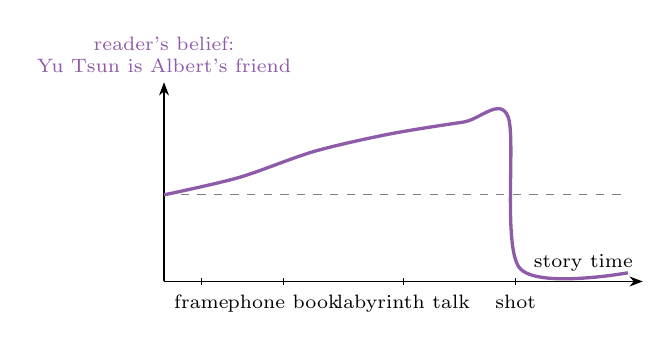
\begin{tikzpicture}[x=0.95cm,y=2.2cm,font=\scriptsize]
  \draw[-{Stealth}] (0,0) -- (6.4,0) node[above left]{story time};
  \draw[-{Stealth}] (0,0) -- (0,1.15) node[above, align=center]{\belief{reader's belief:}\\ \belief{Yu Tsun is Albert's friend}};
  \draw[dashed, gray] (0,0.5) -- (6.2,0.5);
  \draw[very thick, beliefPurple] plot[smooth] coordinates
    {(0,0.5) (1,0.6) (2,0.75) (3,0.85) (4,0.92) (4.6,0.95) (4.75,0.08) (6.2,0.05)};
  \foreach \x/\l in {0.5/frame,1.6/phone book,3.2/labyrinth talk,4.7/shot}
    \draw (\x,0.02) -- (\x,-0.02) node[below]{\l};
\end{tikzpicture}
\\[0.2em]{\tiny\color{gray}illustrative sketch, not data}
\end{column}

\begin{column}{0.42\textwidth}
\footnotesize
\begin{block}{\faRandom\ Devices from the paper}
\begin{itemize}\tightitem
  \item \textbf{flashback}: Liddell Hart frame --- a known delay gets new meaning
  \item \textbf{plot twist}: ``I am your friend'' then the shot ($f_{\text{twist}}$)
  \item \textbf{irony}: Albert says in some futures he is the enemy
  \item \textbf{arc}: terror, hope, calm, murder, triumph
\end{itemize}
\end{block}
\end{column}

\end{columns}
\end{frame}

\begin{frame}{Level 3: the garden is the space of scripts}
\begin{columns}[T,onlytextwidth]

\begin{column}{0.48\textwidth}
\begin{block}{\faCodeBranch\ Ts'ui Pen vs.\ the optimizer}
\begin{itemize}\tightitem
  \item Ts'ui Pen's novel takes \alert{every} branch at once
  \item the optimizer searches the same tree, keeps \alert{one} $\sigma$
  \item two battle chapters, two paths, same victory --- many $\sigma$ satisfy one $f$
\end{itemize}
\end{block}
\end{column}

\begin{column}{0.48\textwidth}
\begin{block}{\faChessKnight\ The chess riddle}
\begin{itemize}\tightitem
  \item the novel is about time, but never uses the word
  \item the reader must \alert{infer} the concept
  \item Yu Tsun never sends the word ``Albert'' either
\end{itemize}
\end{block}
\end{column}

\end{columns}

\slideendspace
\begin{alertblock}{\faLightbulb\ Show, don't tell}
Storytelling = choosing one path through the garden for its effect on what the audience infers.
\end{alertblock}
\end{frame}

% ==================================================
\section{Discussion}
% ==================================================

\begin{frame}{Limits and critique}
\small
\begin{columns}[T,onlytextwidth]

\begin{column}{0.48\textwidth}
\begin{block}{\faExclamationTriangle\ Stated in the paper}
\begin{itemize}\tightitem
  \item scales badly: state, hypothesis and script spaces grow fast
  \item too slow for real-time improvisation
  \item no emotion in the audience model
\end{itemize}
\end{block}
\end{column}

\begin{column}{0.48\textwidth}
\begin{block}{\faBook\ Raised by Borges}
\begin{itemize}\tightitem
  \item \textbf{shared hypotheses}: the Chief must already consider ``a killing encodes a name''
  \item \textbf{noisy one-shot channel} vs.\ full noiseless trajectory
  \item \textbf{unreliable narrator}: the editor's footnote contradicts Yu Tsun
  \item \textbf{remorse} is outside any belief objective
\end{itemize}
\end{block}
\end{column}

\end{columns}

\slideendspace
\begin{alertblock}{\faBalanceScale\ Ethics}
The same machinery that depicts helping can \alert{deceive}: legible vs.\ deceptive motion in robotics.
\end{alertblock}
\end{frame}

\begin{frame}{Discussion questions}
\begin{enumerate}\tightitem
  \item Write an objective $f(\sigma)$ for Yu Tsun. Which term makes the murder beat every other action?
  \item Is the Chief a Bayesian inverse planner? What prior does he need?
  \item Can a branching story like Ts'ui Pen's novel be optimized at all --- or is it the refusal to choose $\sigma$?
  \item Is a good plot twist a script that maximizes $D_{\mathrm{KL}}$ between beliefs at one time step?
  \item Could an LLM serve as the audience model instead of a hand-built inverse planner?
\end{enumerate}
\end{frame}

\begin{frame}[standout]
\centering
\faComments\\
Questions
\end{frame}

\appendix
\begin{frame}[allowframebreaks]{Sources}
\footnotesize
\nocite{*}
\bibliographystyle{apalike}
\bibliography{references}
\end{frame}

\begin{frame}{Appendix: implementation details}
\small
\begin{columns}[T,onlytextwidth]

\begin{column}{0.48\textwidth}
\begin{block}{\faRobot\ Grid world}
\begin{itemize}\tightitem
  \item multi-agent MDP, actions $\{\leftarrow,\rightarrow,\uparrow,\downarrow,\text{stay}\}$
  \item value iteration, hierarchical softmax policies
  \item beam search over scripts, $T=15$ in minutes
  \item all examples use random seed 0
\end{itemize}
\end{block}
\end{column}

\begin{column}{0.48\textwidth}
\begin{block}{\faCogs\ Physics}
\begin{itemize}\tightitem
  \item ``Luxo lamp'' hopper on a hill
  \item SHAC: policy $\pi(s;\theta)$ and value $V(s;\phi)$
  \item box weights 0.1 (light) and 0.5 (heavy)
  \item stumbling: gradient descent on residuals so $V$ dips in $[t_s,t_f]$
\end{itemize}
\end{block}
\end{column}

\end{columns}

\slideendspace
\begin{block}{Code and videos}
\footnotesize \url{https://people.csail.mit.edu/kach/a2i2p/}
\end{block}
\end{frame}

\end{document}
